% !TEX root = ../../thesis.tex

\cleartoleftpage
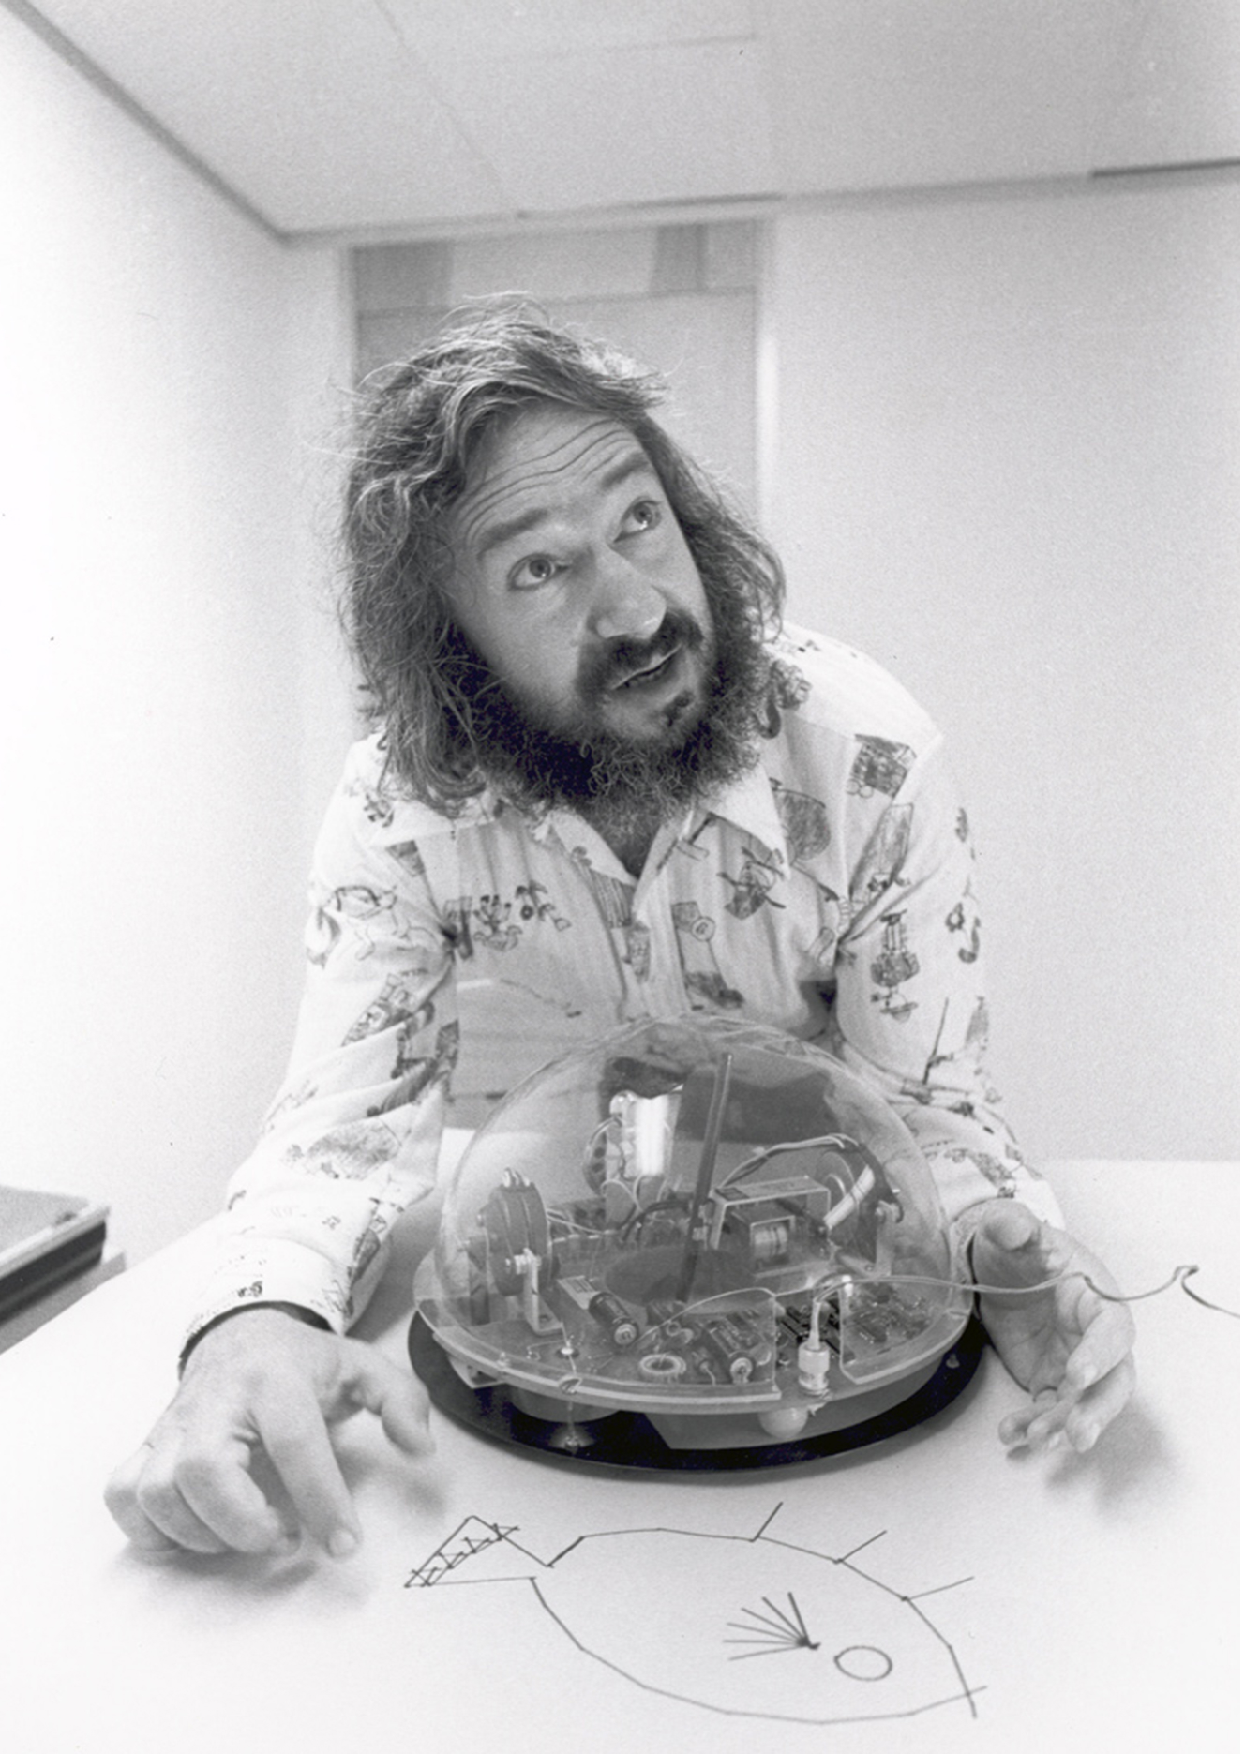
\includepdf{../media/chapter_illustration/seymour-papert.pdf}

\chapter{Education} % (fold)
\label{cha:education}
\cleanchapterquote{New technologies help students navigate the creative thinking spiral.}{Mitchel Resnick}


\section{Introduction} % (fold)

In our modern societies, in particular in France, education is a top priority and a concern for the government and the people. Thus education is central and has to be adapted and relevant to societal evolution. In particular, new technologies have a deep impact on our societies and raise legitimate question and concern~\parencite{plester2008txt}. Also, they can become great vectors to make the education system more efficient and fair.


\textbf{1- Improve access to  and dissemination of education:}

Knowledge is the wealth of humanity and thanks to the very large democratization of the internet, anyone with a connection can now access the whole of humanity’s knowledge in just a couple of seconds. The most famous example is certainly Wikipedia\footnote{\url{http://www.wikipedia.org/}}, a community encyclopaedia with non-stop growing content both in term of quantity and quality. With such a tool, anyone can instantly access  anything one could wish to know, from the history of French "crêpes"\footnote{\url{http://en.wikipedia.org/wiki/Crêpe}} to the explanation of the most famous quantum mechanics principles\footnote{\url{http://en.wikipedia.org/wiki/Schrödinger_equation}}.

In addition to a global encyclopaedia referencing -almost- all of human knowledge, the use of the internet is also changing the way we learn. Indeed, there are more and more websites designed to share free online courses. One of the first successes is the Khan Academy.
The Khan Academy\footnote{\url{https://www.khanacademy.org/}} is an educational website founded by Salman Khan which discusses, along about 2400 videos, principles of math, science, and economics.  It is aimed at helping people master the basics, the humble bread-and-butter equations they encounter in elementary and high school. In addition to the video, the website offers software that tracks the evolution of learning, generates practice problems and uses gamefication to reward performance.
Complementary to Khan's site, which is ruthlessly practical and oriented toward mastering the basics~\parencite{thompson2011khan}, the most famous Universities are beginning to freely diffuse their advanced courses over the internet. We can cite as an example the MIT open course ware (OCW)\footnote{\url{http://ocw.mit.edu/}} or the open Yale courses\footnote{\url{http://oyc.yale.edu/}}.

Finally, the launch of massive open online courses (MOOCs) is currently creating a growing buzz ~\parencite{mackness2010ideals}.

\begin{formal}
    A MOOC integrates the connectivity of social networking, the facilitation of an acknowledged expert in a field of study, and a collection of freely accessible online resources. Perhaps most importantly, however, a MOOC builds on the active engagement of several hundred to several thousand “students” who self-organize their participation according to learning goals, prior knowledge and skills, and common interests.[...]A MOOC generally carries no fees, no prerequisites other than Internet access and interest, no predefined expectations for participation, and no formal accreditation.

    \signed{The MOOC model for digital practice~\parencite{mcauley2010mooc}}
\end{formal}

MOOCs are a recent development in distance education which began to emerge in 2012~\parencite{pappano2012year}. In France, a first step was taken at the end of October 2013 with the creation of the website France Université Numérique\footnote{\url{http://www.france-universite-numerique.fr/}}, which tries to promote the development of MOOC teaching in France.


\textbf{2- Teaching people to be comfortable with and aware of the digital world}

A commonplace is to refer young people as "digital natives". Yet their apparent fluency with digital technologies (e.g. smartphone and computer) does not mean they actually understand the technology as well as the hidden implications, in particular about the privacy.

\begin{formal}
    Although young people interact with digital media all of the time, few of them can create their own games, animations, or simulations. It is as if they can "read" but not "write".

    \signed{Scratch: Programming for Everyone~\parencite{resnick2009scratch}}
\end{formal}

To introduce computer concepts to children, MIT Media Lab developed Scratch~\parencite{resnick2009scratch} forked by Berkeley into Snap, an extended reimplementation of Scratch that makes it suitable for a serious introduction to computer science for high school or college students. With its block interface, it allows to code by combining blocks like Lego.

\begin{formal}
    Digital fluency requires not just the ability to chat, browse, and interact, but also the ability to design, create, and invent with new media~\parencite{resnick2008sowing}. To do that, you need to learn some type of programming. The ability to program offers many important benefits: it greatly expands the range of what you can create (and how you can express yourself) with the computer, while also expanding the range of what you can learn. In particular, programming supports the development of “computational thinking,” helping you learn important problem-solving and design strategies (such as modularization and iterative design) that carry over to non-programming domains. And since programming involves the creation of external representations of your problem-solving processes, programming provides you with opportunities to reflect on your own thinking and even to think about thinking itself~\parencite{disessa2001changing}

    \signed{Scratch: Programming for Everyone~\parencite{resnick2009scratch}}
\end{formal}


\textbf{3- Using robots as new pedagogical tools}

Robots have a great potential to become ideal tools for teaching a wide range of engineering disciplines. Indeed, robots are intrinsically multidisciplinary objects embedding technology from diverse fields, among them computer science, mechanics, electronics or signal processing.
The current low-cost projects emerging from the makers revolution\parencite{anderson2012makers} such as Arduino\footnote{Open source electronics boards}~\parencite{mellis2007arduino}, Raspberry Pi\footnote{Low cost micro Linux computer}, and 3D printing bring the tools needed to create robots at a cost that is compatible with the funding available in education. Now the technology lets students create or modify actual robots, a great motivational tool because they permit instant application in the real world, giving a meaningful context favourable for constructivist teaching~(\cite{palincsar1998social}, \cite{papert1991situating}).
There are already several great success stories such as the e-puck robot~\parencite{mondada2009puck} which specifically targets engineering education at university level or Thymio II adapted for teaching robotic and computer science in primary education~(\cite{riedo2012two}, \cite{riedo2013thymio}).


\subsection{Education and the Poppy project} % (fold)

The Poppy platform was initially designed for research purposes and even more specifically for studying biped locomotion and human-robot interaction. However, it has been designed with open science goals in mind, both to share our research and create tools for researchers. As we are convinced of the need for multidisciplinary contributions in order to improve the state of the art in the robotics field, we decided right from the beginning to use and create modern and easy-to-use tools. This choice has strongly affected the way we designed our platform. Indeed, being simple to use, easily reproducible and hackable, modular, 3D printable and as plug 'n play as possible lead to the development of hardware (Poppy) and software (pypot) tools that can be also used by non-expert people.

Thus Poppy meets a growing societal need: education and training in technologies combining computer science, electronics and mechanics, as well as a training tool for the emergent revolutionary 3D printing process. Since October 2013 (open source release), we have been contacted by several Fablabs, universities, engineering schools and even high schools. We have had the opportunity to meet with educational teams and it appears they are looking for new motivational tools for group projects.

In this context, the Poppy platform appears well suited. Indeed, it integrates advanced and yet easily accessible techniques (3D printing, Arduino, Python) in an embodiment that motivates students and the wider public. With its openness, design and rather low-cost, Poppy is highly hackable and provides a unique context for learning and experimenting with these technologies in a Do-It-Yourself (DIY) way.

Several experiments with Poppy in middle and high schools, science museums and Fablabs in France and abroad are already underway and will be discussed in the upcoming sections.


\section{Educational exploration with Poppy in high school} % (fold)

After the artistic residency that took place in the chapel at the Saintonge Sainte Famille high school (see chapter~\ref{cha:art}), some teachers have become interested in the educational potential of the Poppy project and would like to integrate it as a common thread into the school year.

Poppy was initially designed for research purposes and seems to be also adapted for higher education. Yet using Poppy in secondary education seems excessive as it is expensive and the use of high quality servo-actuators is not really justified. However, the experience with high-school students is still interesting and we accepted this opportunity to do a pilot experiment.

\textbf{For the teachers}, the main goal was to gain experience of using such tools in a project context and evaluate the potential and limitations for educational purposes.

\textbf{For us}, we were interested in the reaction of young students to Poppy and in getting an opinion on the relevance of Poppy for education at this level. Also, it was a real crash test of our design (hardware and software) in non-experienced hands and outside the laboratory.

\subsection{Proceedings} % (fold)

The experiment took place in the Saintonge Sainte Famille high school on May 26th \& 27th, and involved near 40~\emph{première STI2D} students (equivalent to UK Year 12) preparing a professional baccalaureate and three teachers (\emph{"Energy and environment"}, \emph{"Architecture and construction"}, and \emph{"Digital information systems"}).
It was organized as a workshop in three 4-hour sessions. The last two hours were dedicated to oral presentations in the lecture hall allowing students to share their experiences and work (see \figurename~\ref{fig:saintonge_support} and \figurename~\ref{fig:saintonge_demonstration}).

For this first pilot experiment, we decided to reduce the cost by using only a sub-part of the whole Poppy. For us the most relevant part for high-school students was the upper body (thorax, head and the two arms), because it avoids to work on complex sensory-motor behaviours such as balancing and walking while keeping the expressive potential of Poppy. The total cost of Robotis Dynamixel motors, electronics and 3D printing service was \texteuro2500 (20 \% tax included), the BOM list is available in the appendix~\ref{appendix:education_bom}.


Students were assigned several sub-tasks that we will describe in the following sections.


\subsection{Assembling Poppy} % (fold)

The assembly of Poppy was divided in three groups: one was doing the assembly of the thorax and the head (4 motors) and two others for each arm (3 motors). At the end of the first day the half-Poppy was assembled (see \figurename~\ref{fig:saintonge_assembly}) with little difficulty.

\begin{figure}[tb]
\centering
    \subfloat[][Motor assembly and configuration]{\includegraphics[width=0.48\linewidth]{saintonge_assembly1.jpg}}
    \hfill
    \subfloat[][Thorax assembly]{\includegraphics[width=0.48\linewidth]{saintonge_assembly2.jpg}}
    \hfill
    \subfloat[][Arm assembly]{\includegraphics[width=0.48\linewidth]{saintonge_assembly3.jpg}}
    \hfill
    \subfloat[][Poppy almost finished, only the face is missing]{\includegraphics[width=0.48\linewidth]{saintonge_assembly4.jpg}}
    \caption{Poppy was assembled by 3 parallel working groups divided into thorax + head and the 2 arms. At the end of the first day, the half-Poppy was assembled and functional. }
    \label{fig:saintonge_assembly}
\end{figure}

However, as we will discuss in more detail in the upcoming section~\ref{sec:education-lessons}, we experienced some difficulties with the high school internet connection and all documentation is online\dots So it was unfortunately rather difficult to evaluate if our documentation was clear enough for high school students. Yet, from that we experienced explaining the "how-to" guide and it appears we need highly detailed documentation for the very first steps. General guidelines seem to be enough to achieve a well-assembled Poppy robot.

\subsection{Python programming with pypot}

Two working groups were dedicated to learning basic Python programming with pypot (see \figurename~\ref{fig:saintonge_software}). The teacher had selected these students because of their enthusiasm for computer science. Indeed when they heard about the Poppy project several weeks earlier, they became interested in Python and began to look for further information on the internet.

The first hours of the software workshop were complicated. The school computers were not outdated but were running on Windows and used by a lot of different people, so configurations were not consistent between machines and sometimes rather exotic. The installation of the necessary tools (Python + packages + text editor) was particularly long and painful. We will come back to this point in the section~\ref{sec:education-lessons}.

\begin{figure}[tb]
\centering
    \subfloat[][One software working group discussing pypot with their teacher]{\includegraphics[width=0.48\linewidth]{saintonge_soft1.jpg}}
    \hfill
    \subfloat[][The two software groups discussing Poppy's configuration file]{\includegraphics[width=0.48\linewidth]{saintonge_soft2.jpg}}
    \hfill
    \subfloat[][Experimentation through trial and error]{\label{fig:saintonge_motivated_software_guy}\includegraphics[width=0.48\linewidth]{saintonge_soft3.jpg}}
    \hfill
    \subfloat[][Transmission of knowledge between classmates]{\label{fig:saintonge_knowledge_transmission}\includegraphics[width=0.48\linewidth]{saintonge_soft4.jpg}}
    \caption{High-school students discovering programming with Python and the pypot library}
    \label{fig:saintonge_software}
\end{figure}

Once the desktops were set up, students took a look at the basic pypot tutorials\footnote{\url{http://poppy-project.github.io/pypot/tutorial.html}}. They first tried to control one Dynamixel motor (reading/setting positions). Then they used a group of motors (each with one Poppy arm) and we introduced the pypot robot configuration feature. At this point they were able, thanks to the basic pypot tutorial, to create a robot with specific motor configurations and make it move by setting direct goal positions or using sinus trajectories. This improvised complexity slope lead them to a good understanding of the very basic features of pypot and Dynamixel motor properties in just 2 hours and without any previous Python experience.

The hardware groups then assembled Poppy, the software group modified Poppy's configuration file and adapted it to their own Poppy. At the end of the first day, the two groups were able to make their Poppy move.

The software team continued their work the next day, trying to create more complex behaviour. One participant (see \figurename~\ref{fig:saintonge_motivated_software_guy}), managed to create on his own (we did not write a single line of code) the copy-arm behaviour we showed in the Poppy overview video\footnote{http://vimeo.com/poppyproject/poppyoverview}. Then he explained how he did it to his classmates (see \figurename~\ref{fig:saintonge_knowledge_transmission}).

After learning how this behaviour was achieved, another group decided to make Poppy clap its hands. By trial and error they managed to make the basic movement by using sinus. This self-exploration required an understanding of what a variable is and how a sinus acts and they experimented on their own with the different sinus properties such as frequency, amplitude and even offset. As Mitchel Resnick explained in~\parencite{resnick2009scratch}, here the meaningful context of making a robot move arouses the students’ curiosity in mathematics and computer science concepts.



\subsection{Design of a Poppy's support in Solidworks} % (fold)

As we were only building the very upper part of the robot, several students worked in pairs to design a wheeled platform supporting their own Poppy version. The teacher’s instructions were to create a mobile support for their Poppy with enough room to include batteries and a computer.

For most of them it was their first experience using parametric modelling tools. However, the final result (see \figurename~\ref{fig:saintonge_support}) is quite impressive. All working pairs managed to finish the basic idea of their design choices and integrate the Poppy robot.

One really interesting point is that they all chose a different design to make their support structure move. Some used caterpillar tracks, others four or two wheels and one freewheel. The Poppy robot gives a pretext for creation and leaves students free to explore.

\begin{figure}[tb]
\centering
    \subfloat[][Caterpillar design]{\includegraphics[height=3cm]{saintonge_support1.jpg}}
    \hfill
    \subfloat[][Four independent wheel design]{\includegraphics[height=3cm]{saintonge_support2.jpg}}
    \hfill
    \subfloat[][Two motorized and a freewheel]{\includegraphics[height=3cm]{saintonge_support3.jpg}}
    \caption{Students of the design support work group explain their choices to others.}
    \label{fig:saintonge_support}
\end{figure}

Of course,  they did not manage to produce the prototype within the two days but it showed to the teaching staff what kind of project they could launch if they had a 3D printer to produce the student works.

\subsection{Documentation } % (fold)

Finally, the other students were in working groups in charge of reporting the different workshop activities. They had to take pictures of the robot assembly and capture an overall view of the project to extract meaningful information for building SYSML diagrams with MagicDraw. They also had to practice English and report on the translation of technical words in a robotic context.

The students of these groups were far less enthusiastic than the others, some even discreetly sneaked into other workshops. Of course, building and programming a robot is  far more fun than reporting it. This shows some limitation of a project such as Poppy: there is not enough work for lots of students, introducing inequalities in the repartition of tasks.

\subsection{Results} % (fold)

The student team managed to assemble a fully functional Poppy. Groups working on control were able to make a live demo of Poppy moving at the end of the workshop (see \figurename~\ref{fig:saintonge_demonstration}).

\begin{figure}[tb]
\centering
    \subfloat[][First Poppy's moves drew particular attention.]{\includegraphics[height=4.3cm]{saintonge_poppy_first_moves.jpg}}
    \hfill
    \subfloat[][Live demonstration of the robot behavior students created]{\includegraphics[height=4.3cm]{saintonge_demo1.jpg}}
    \caption{After finishing the hardware assembly, students began to make Poppy move using the pypot library. They manage in just few hours to create impressive movement and behaviour despite no previous development experience with Python.}
    \label{fig:saintonge_demonstration}
\end{figure}

This experience was very instructive on several aspects relative to the usage of Poppy for education purpose. In particular, it raises some problems we would have never thought about without a "real world" experimentation in a school environement. All these points will be largely discussed in the section~\ref{sec:education-lessons}.

\newpage
\section{Fablab workshop} % (fold)
\label{sec:poppy_universience}

On March 22nd \& 23rd 2014, UniverSciences\footnote{Paris museum of sciences and technologies} organized a hackathon for the general public on the assembly of a Poppy robot (see \figurename~\ref{fig:universience_workshop}).
It involved 21 robotic enthusiasts (aged from 23 to 46) with various backgrounds (informatics, electronics, physics, sociology, mechanics, architecture).

Participants were divided into several working groups during the two days. While a group was dedicated to the actual assembly of Poppy, others were exploring how to program the robot in Python or working on designing and 3D printing hardware improvements. During the weekend, nearly 100 visitors came to visit the workshop and some of them participated in the hackathon.

This hackathon was really interesting for us because it was the first time a Poppy was assembled without any member of the team present, therefore we were able to see what happens when people are left alone with just online documentation, the forum and the robot parts.
We were giving live support through the forum (see associated topic\footnote{\url{https://forum.poppy-project.org/t/poppy-project-at-la-cite-des-sciences-et-de-lindustrie}}) and at the same time completing the documentation\footnote{\url{https://forum.poppy-project.org/category/documentation}} as problems occured.

\begin{figure}[p]
\centering
    \subfloat{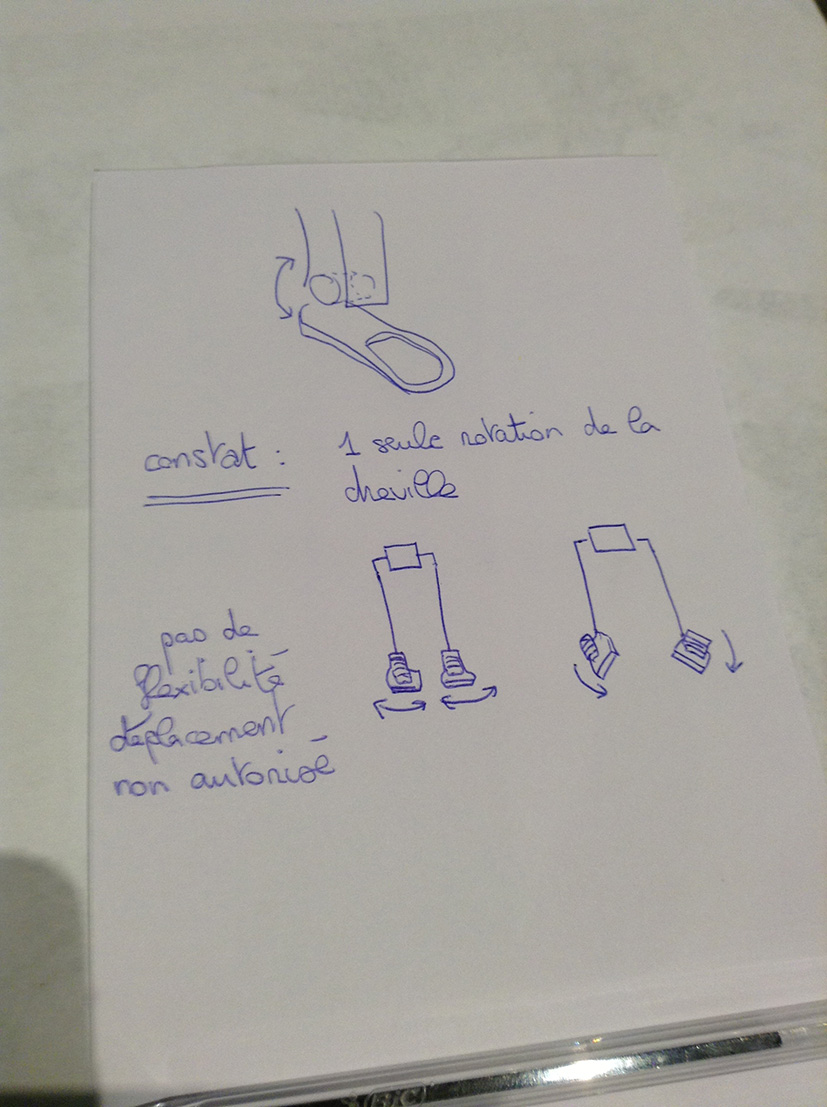
\includegraphics[height=5cm]{hackathon_conception1.jpg}}
    \hfill
    \subfloat{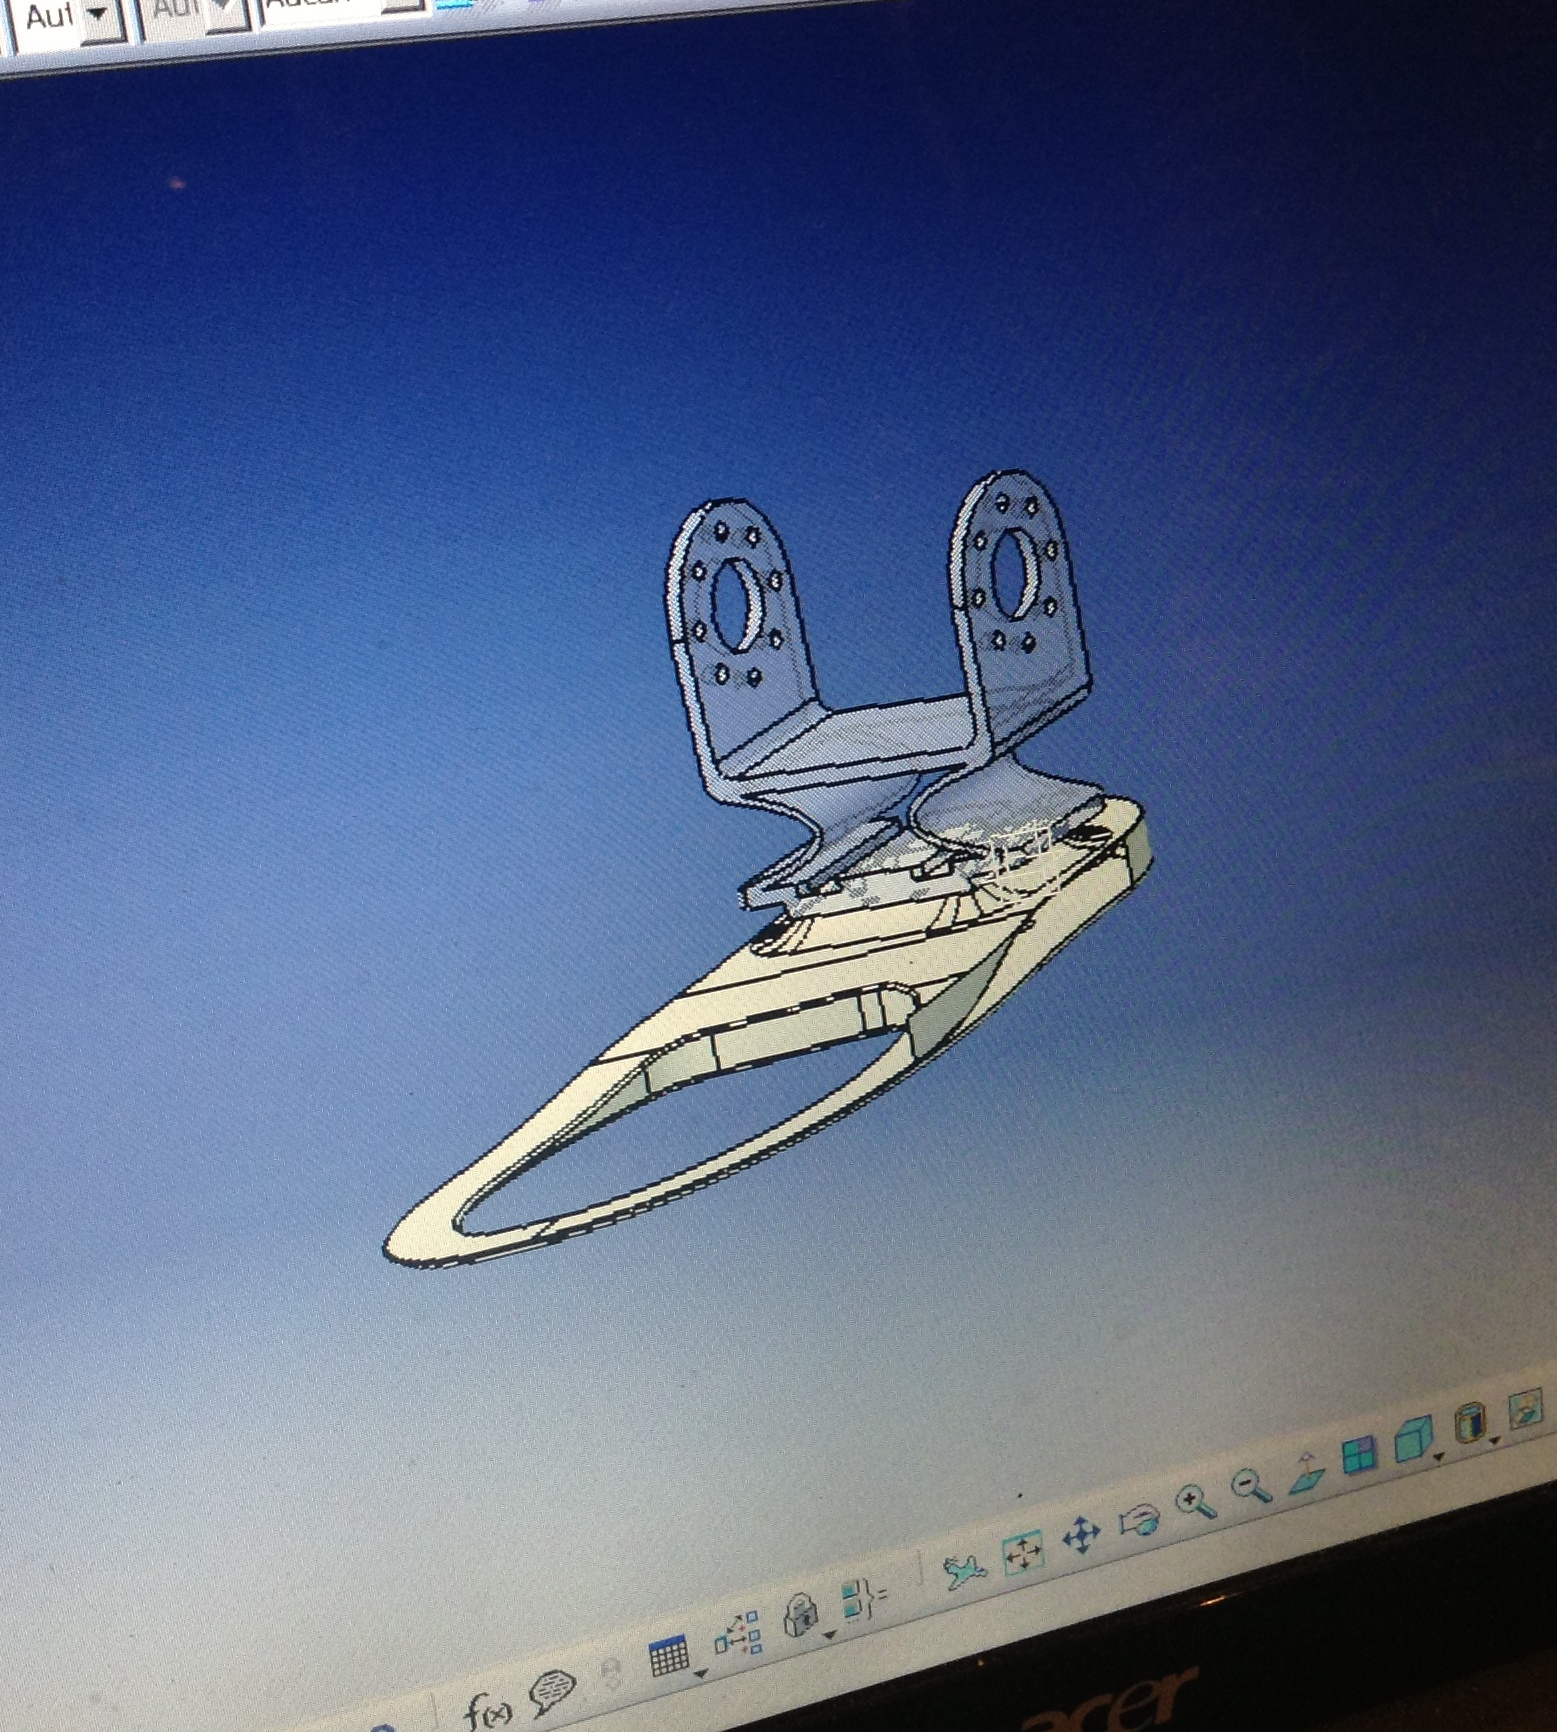
\includegraphics[height=5cm]{hackathon_conception2.jpg}}
    \hfill
    \subfloat{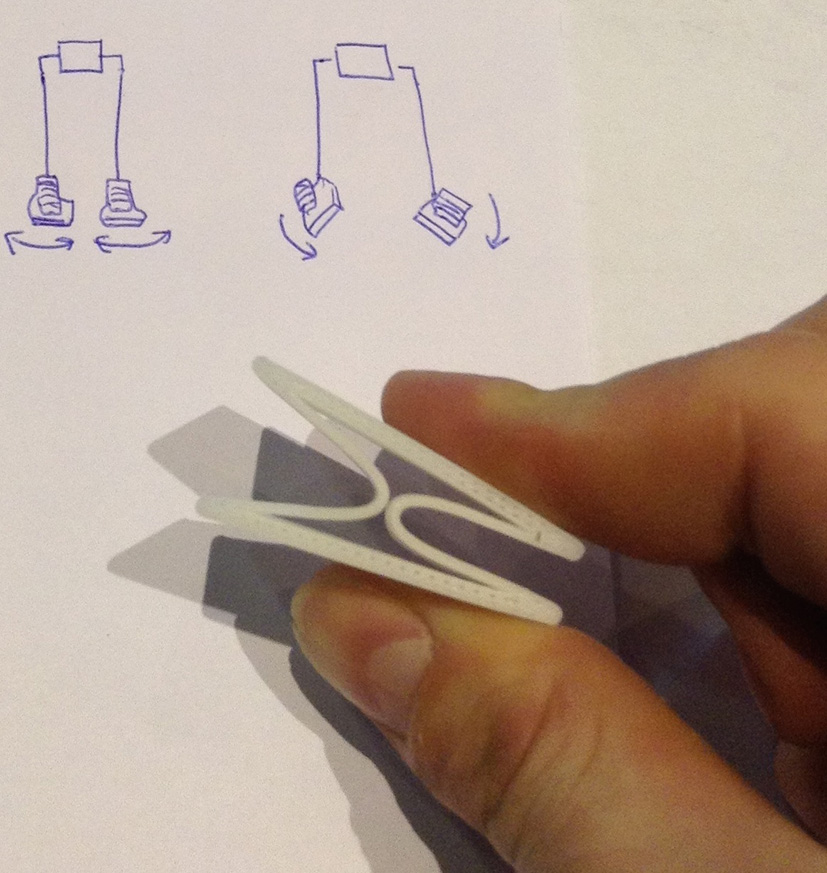
\includegraphics[height=5cm]{hackathon_conception3.jpg}}\newline
    \subfloat{\includegraphics[height=4.63cm]{hackathon_assembly1.jpg}}
    \hfill
    \subfloat{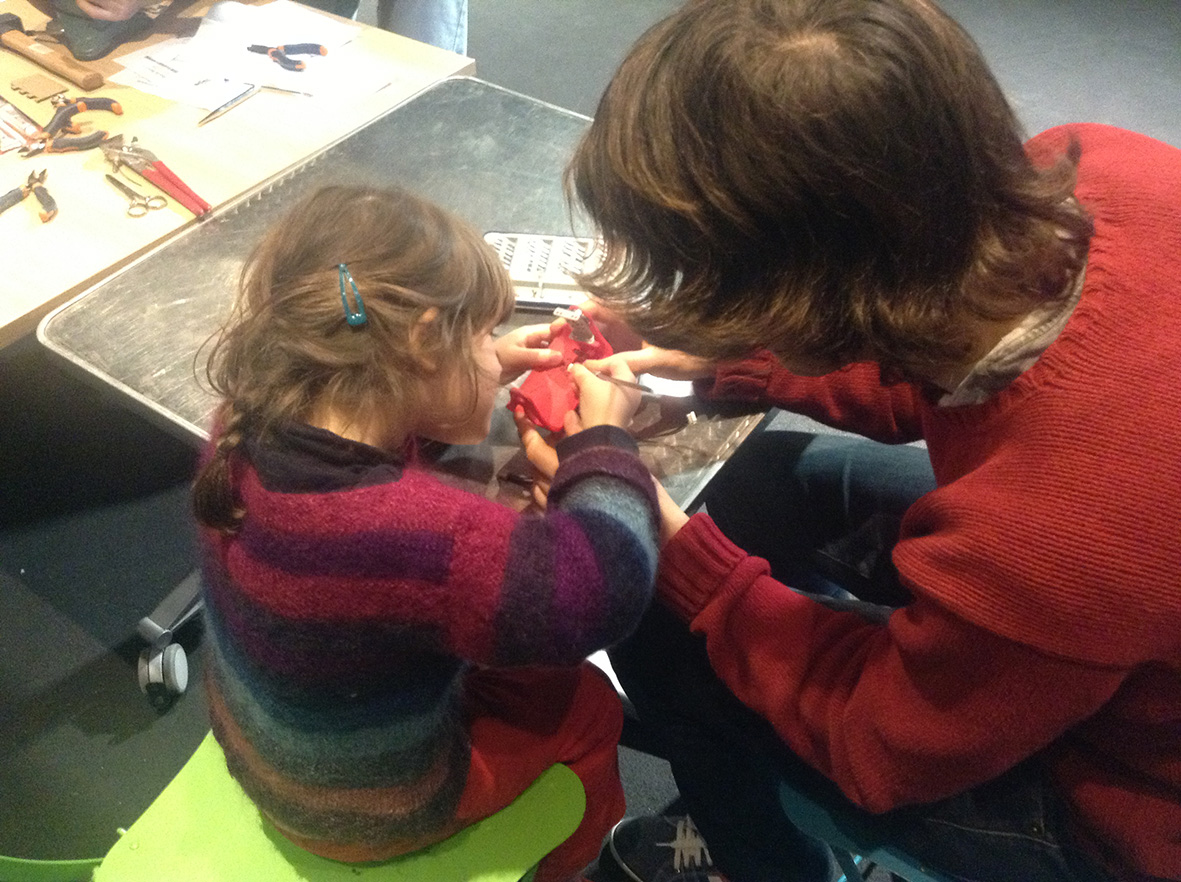
\includegraphics[height=4.63cm]{hackathon_assembly2.jpg}}\newline
    \subfloat{\includegraphics[height=4.95cm]{hackathon_assembly3.jpg}}
    \hfill
    \subfloat{\includegraphics[height=4.95cm]{hackathon_last_screw.jpg}}\newline
    \subfloat{\includegraphics[height=6cm]{hackathon_poppy_assembled.jpg}}
    \hfill
    \subfloat{\includegraphics[height=6cm]{hackathon_first_trial.jpg}}
    \caption{Several photos taken during Poppy's assembly for the UniverScience hackathon.}
    \label{fig:universience_workshop}
\end{figure}

The support was needed to help the team and showed us some points on which we have to improve in order to make Poppy easier to use and assemble:
\begin{description}
    \item[Cable routing:] if mounted too soon, some motors have to be dismounted in order to be connected, which can be frustrating.
    \item[Dynamixel motors:] require several critical steps which can cause painful difficulties afterwards, among them:
    \begin{itemize}
        \item The horn of the motor has to be correctly oriented to set the initial position but can be only mounted once.
        \item The configuration of each motor needs to be set individually before being assembled. The motor has a unique ID for communication set to 1 by default.If all motors are plugged with the same ID, neither communication nor configuration is possible.
    \end{itemize}
    \item[Screw size:] This is something we had not considered but it is actually difficult for people to distinguish the differences between two and where they should go.
\end{description}

Despite these minor difficulties, this group of new users, self-trained using only online community tools were able to build the whole robot from scratch and make it move using the pypot library. Eventually, two young students  had an idea: 3D printing an ankle that could give some articulated movement to Poppy's feet. They designed a new original semi-passive solution for the ankle joint as well as a robot helmet that was 3D-printed and assembled within the time of the workshop (see \figurename~\ref{fig:universience_workshop}). Also the feedback we received from the mediation team was really good and they are enthusiastic to repeat this kind of event.


\begin{figure}[tb]
\centering
    \subfloat{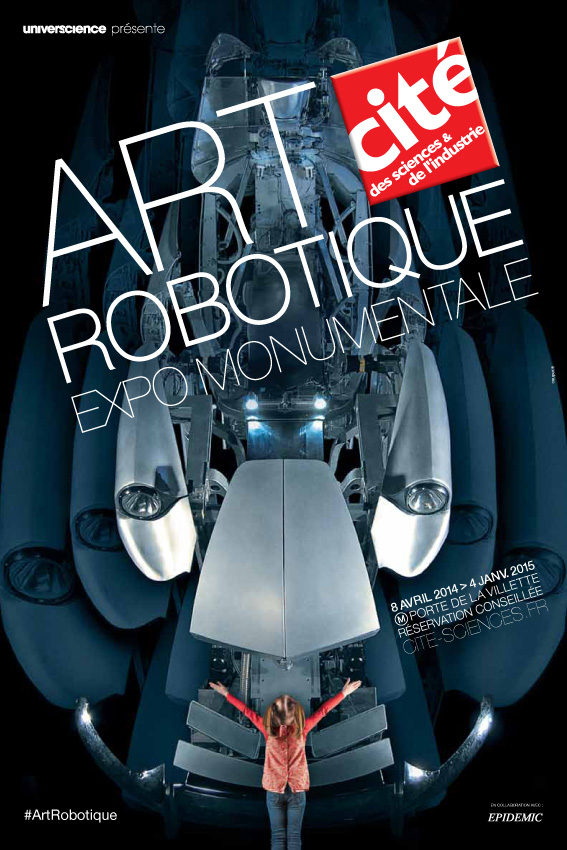
\includegraphics[height=6cm]{art-robotique_universcience.jpg}}
    \hfill
    \subfloat{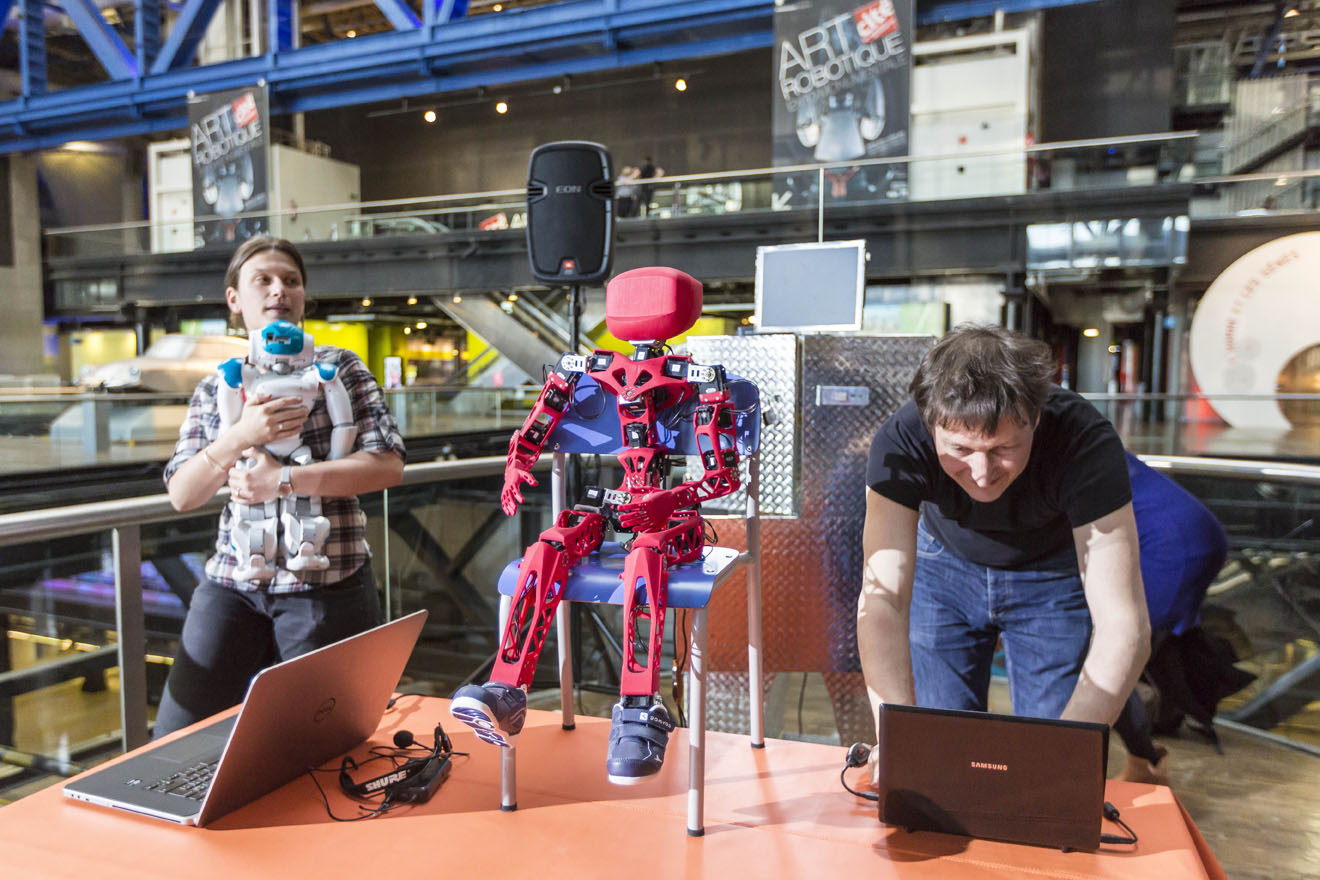
\includegraphics[height=6cm]{poppy_demo_universcience.jpg}}
    \caption{Currently Poppy is used by UniverScience for mediation acts along the "Art Robotique" exposition.}
    \label{fig:universcience_art}
\end{figure}

Since this hackathon, Poppy has been used by the UniverSciences Fablab, but also for activities and animation aside from the "Robotic Art" exhibition (08/04/2014 to 04/01/2015) \figurename~\ref{fig:universcience_art}. It formed part of the opening of the exhibition on April 8th, and is part of the science show "l'ère des Robots" (The Robots Era)\footnote{\url{http://www.cite-sciences.fr/fr/au-programme/expos-temporaires/art-robotique/activites-associees/}}.


% \cleardoublepage

\section{Lessons learn} % (fold)
\label{sec:education-lessons}

These experiments were really instructive as we had the chance to do a real crash-test in ecological conditions: a group of people left alone to build a complex robot in a Fablab style environment and real students in their high school and with their own equipment. As we personally took part in the workshop in the high school, this section resuming the educational interest will be more focused on this experiment.

For example, Mitchel Resnick cited the experience a teacher had while using Scratch for a school project~\parencite{resnick2008sowing}:
\begin{formal}
    There is a buzz in the room when the kids get going on Scratch projects. Students set design goals for their projects and problem-solve to fix program bugs. They collaborate, cooperate, and co-teach. They appreciate the power that Scratch gives them to create their own versions of games and animations.

    \signed{Karen Randall, teacher at the Expo Elementary School in~\parencite{resnick2008sowing}}
\end{formal}

This description closely resembles my experience with the high school students. We were really surprised and pleased at how the students were able to switch from a pyramidal way of learning, where they are passive and expect the teacher to transmit knowledge, to a horizontal one or even a bottom-up one, where students are proactive and ask the teacher for explanations, use these to understand novel concepts then transmit them to their classmates.

This experiment turns out to be much more instructive than expected and taught us several lessons:

\textbf{1- A robotic project is very motivating:} the goal of having their own "cool" robot moving was a really impressive motivational fuel. Students were not discouraged by the difficulties that cropped up on the path toward achieving their goal. Also they had a positive way of trying to overcome them. Surprisingly, they did not seem bored by all the inconveniences that occurred such as installing tools on machines, Python syntax tricks or remounting an assembly because they had made a small mistake. Actually, the teacher seemed far more bothered than his students.

\textbf{2- Robots provide a meaningful context, conducive learning mathematical and computer science concepts:}

Problems that crop up when making and controlling a robot require the use of math and students see in this the tools needed to reach their goal. They are learning math because it is on the way to achieving a “cooler” and more rewarding goal. In this pilot experiment, the students were from a professional baccalaureate, typically the kind of students saying they are not "born mathematicians" and so will never succeed in doing it. However, while trying to control Poppy, especially making it clap, they were confronted with mathematical problems and used sinusoidal signal to resolve them. Using Poppy they were able to see, immediately and in real life, the usefulness of sinus and eventually began to explore on their own the role of each parameter (amplitude, frequency, phase, offset).

The same effect can be observed in teaching computer science and programming. Indeed, having to deal with strange syntax rules, complex commands and austere interfaces is discouraging. Using robots makes the programming experience much different. You are not studying computer science to print characters on a black system console, but you are using programming to make a robot move!
During the experience with the high school students we saw two main advantages. Firstly, the motivation of making a robot move helps students to overcome the syntax tricks problems. Secondly, teaching Object-oriented programming (OOP) using actual object is far easier. Indeed, understanding that a motor is an object with properties and functions is really meaningful.


\textbf{3- Poppy is open source, it can be hacked and adapted to specific needs:}
The fact Poppy is at the same time open source, 3D printed and “cool” definitely makes it  an ideal application for education. Its design catches the students’ attention while the free use of all its sources allows teachers to create educational content based on exploration and understanding of the state of the art and lets students express their creativity by hacking the platform.


Also, because Poppy is modular, it allows teachers to adapt its use to their needs. Here, it was possible to only take one part of the robot and use the student’s creativity to create the missing elements. This kind of usage would not be possible if Poppy was a commercial and closed robot.

\textbf{4- Do not rely on educational equipment:}
The internet access was really bad, so slow that our forum could not be displayed. Also, even if school computers are quite up-to-date, they are used by a lot of different users with various levels of expertise and potentially have incompatibilities or odd configurations. So we cannot expect to find a working environment close to the one we have in our labs.
We have to either ensure before the workshop that every desktop is ready or use tools more robust to system configuration issues.

\textbf{5- Well-designed and stand-alone IDE is needed.}

The previous point showed us that the current way of working with Poppy was not adapted to its use in high school. Indeed, we lost almost all of the first 4-hour session just trying to set up a development environment allowing the use of the pypot library. We eventually gave up on certain high-school machines and we stopped when we got the minimum required tools. However, there are complementary tools such as ipython notebook that greatly improves the convenience when programming in Python.

Thus eventually, high-school students managed to develop complex behaviour with Poppy but the teacher had pre-selected them on the basis of their enthusiasm about computer science. Students without prior excitement would probably give up when faced with so many system setup difficulties.

This problem led us to look for improvements and we eventually found an interesting way to overcome these setup issues. The week after, we submitted a project proposal to the Aquitaine Region funding call on the design of a development environment adapted to the use of Poppy in educational context. We will describe this project more in future work (see section~\ref{sec:education-future-work}).


\textbf{7- Content should be translated into the native language:}

The Poppy project was initially a research project and English is the only language used for information and documentation. Yet this choice is a real problem in the educational world. In France, a large number of people are either not fluent or completely unable to speak and understand English. Of course, the younger the students,  are, the less they are comfortable they are with foreign languages. In addition, teachers’ English level is also pretty poor and so the fact that the information we give is in English is a stumbling block to the diffusion of Poppy in the French education system.


\section{Discussion} % (fold)

Open source 3D-printed robots can help in the creation of meaningful contexts allowing people and students to explore several aspects of science, among them, computer science, mechanics and electronics. In particular, the use of Poppy can be a great gamification tool for scientific mediation and educational purposes.

As it allows people to explore by themselves the basics of robotics, Poppy confront users with the use of programming and mathematical concepts which can raise the awareness of the general public about complex scientific challenges and the usefulness of such technical sciences, often studied in a meaningless context.
Poppy is not a "black box". It has to be assembled and even if it is quite simple to program, people need to understand the basics of programming and then find out by trial and error how to achieve a desired behaviour. Thus, using Poppy leads to the use of the scientific synthetic methodology "understanding by building" and a constructivist learning approach, which are great methods for both fostering critical thinking and creating deep reflexions on the understanding of nature.

Also for a small amount of time, students are scientific researchers lost in an open field of exploration. It is a really great way of introducing people to scientific thought, doing experiments by trial and error, trying to understand how to achieve a desired goal, creating models using math or algorithms.

However, even if the two experiments conducted showed a high potential for Poppy’s societal impact on education, there are still several limitations:

Firstly, Poppy is low cost for research labs but it is still too expensive to have a real impact on the education system. Its current cost makes it accessible only to some privileged high schools. Also, even in the high schools that can afford such a robot, it is only possible to have one or two which leads to inequalities in the project course. A few students have the chance to build the robot or make it move while others are passive and cannot take part in the activity.

However, using such high quality actuators is not really relevant for educational uses, at least before baccalaureate. While the humanoid shape seems to really have an impact on the students’ motivation, the fact Poppy is tall and compliant is not a real need. We could and should definitely propose a cheaper alternative more adapted to elementary and high schools. Poppy being still relevant in universities, engineering schools and of course research labs.

Secondly, the way   the robot is controlled is not adapted to an educational context. Having to spend time installing each package needed and then figure out why the system crashes is not really interesting or relevant for students. They should instead spend time on programming and using the robot. Also, there are successful educational projects such as Arduino~\parencite{banzi2009getting} and Thymio~\parencite{shin2014visual}  propose such plug 'n play IDE (see \figurename~\ref{fig:eductationnal IDE}).

\begin{figure}[tb]
\centering
    \subfloat[][Arduino]{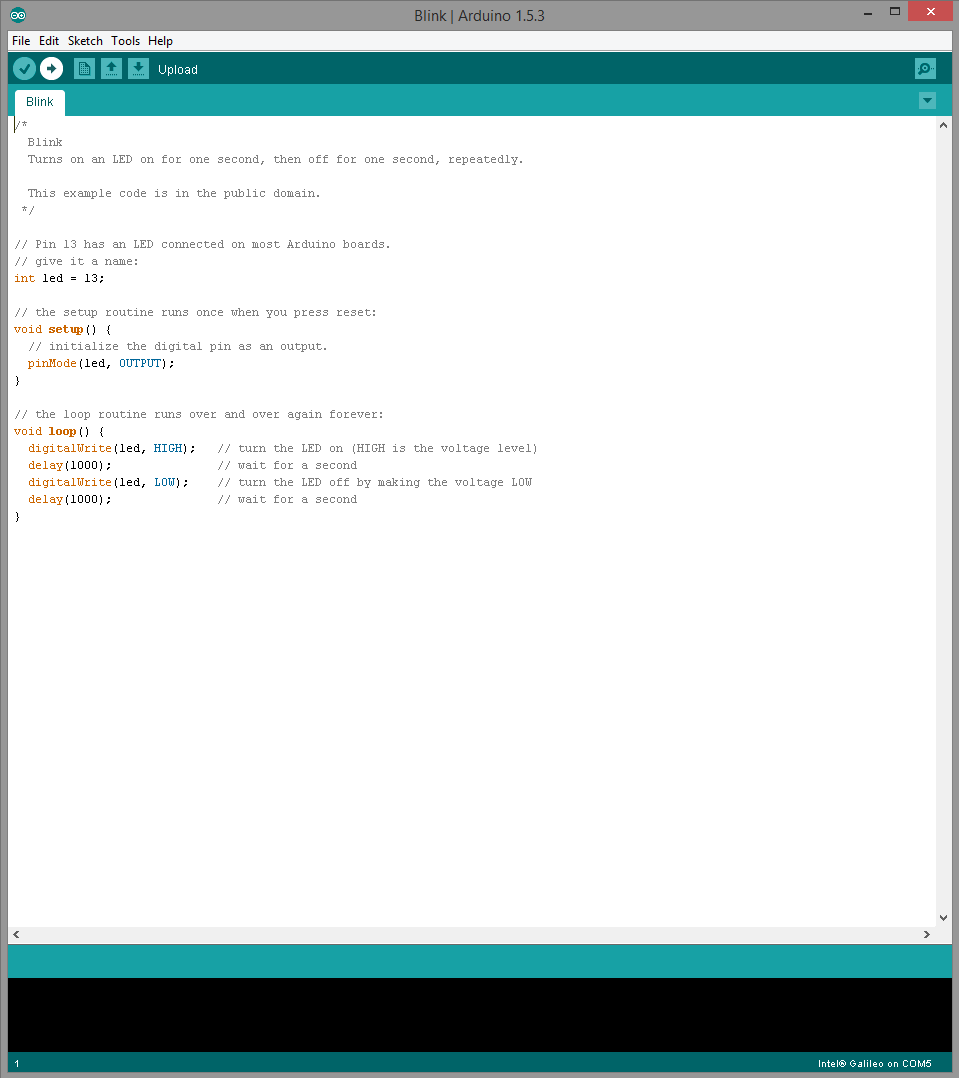
\includegraphics[height=6cm]{arduino_IDE.png}}
    \hfill
    \subfloat[][Thymio 2 IDE]{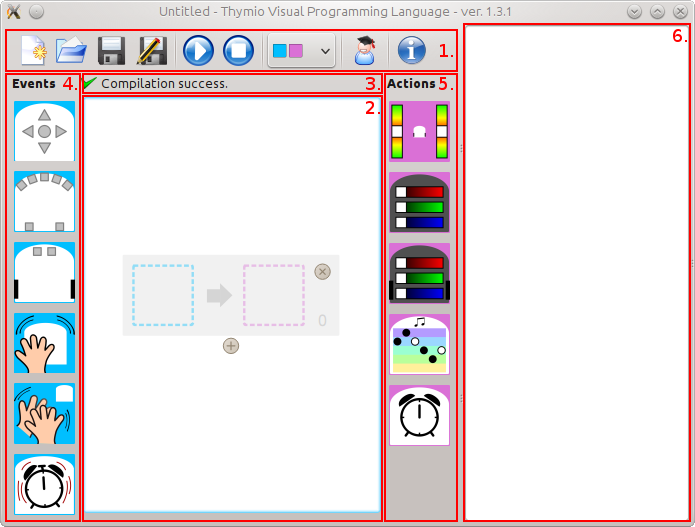
\includegraphics[height=6cm]{thymio_IDE.png}}
    \caption{Arduino and Thymio are stand-alone IDE allowing to have plug 'n play devices, immediately useable right out of the box. Also, the user interface is done to make writing and debugging code easy. Creating great IDE seems essential for success in education.}
    \label{fig:eductationnal IDE}
\end{figure}


Finally, we should be careful that the activities associated with Poppy are not only playful but have a real educational impact. To do so, actual teachers need to create educational content. Of course it is easy to get the students attention for 2 days with a project as fun and playful as Poppy but creating relevant content running as projects along a whole school year is far more challenging.

Confronted with these three points, we found promising technical solutions and we set up a partnership with educational local actors to propose a project to the Aquitaine Region in order to get the resources needed for development.


\section{Future work} % (fold)
\label{sec:education-future-work}

As we explained previously, experiments involving Poppy have shown potential for educational application. However, given the cost of Poppy, the complex setup to run pypot and the lack of educational content, the relevance of Poppy in high schools and first years of universities is still questionable.

So we decided to address these needs and we launched a partnership with a famous engineering school (ENSAM) and a high school (Saintonge Sainte Famille) working towards the creation of educational content and user experimentation in  real contexts.

The Poppy Education project aims to develop, utilize and disseminate a teaching platform based on the use of Poppy for integrated learning of computer sciences and engineering. In particular, it aims to provide:
\begin{itemize}
    \item An open source integrated development environment (IDE) based on web technologies with an embedded Python interpreter. This application can be stand-alone and will allow both the sharing and deployment of educational resources based around the use of the robot, and a friendly interface to program and monitor it.
    \item Design a mini version of the current Poppy robot. Using \$20 Robotis Dynamixel XL320, it would be possible to build a 30cm tall 3D-printed Poppy for around \$500.
    \item educational content using this environment, Poppy, and Poppy mini in real situations with high school and bachelor courses (thanks to our partnership with ENSAM and Aerocampus).
    \item the dissemination of these educational tools under open source and Creative Commons licenses.
    \item the translation of the software, the documentation and educational content in French and English. Other language translations will be done with external contributions.
\end{itemize}
